\documentclass[10pt,twocolumn,letterpaper]{article}
\usepackage{array}
\usepackage{statcourse}
\usepackage{times}
\usepackage{epsfig}
\usepackage{graphicx}
\usepackage{amsmath}
\usepackage{amssymb}
\usepackage{booktabs}
\usepackage{multirow}
\usepackage{hyperref}
% Include other packages here, before hyperref.

% If you comment hyperref and then uncomment it, you should delete
% egpaper.aux before re-running latex.  (Or just hit 'q' on the first latex
% run, let it finish, and you should be clear).

\statcoursefinalcopy%

\setcounter{page}{1}
\begin{document}


%%%%%%%%%%%%%%%%%%%%%%%%%%%%%%%%%%%%%%%%%%%%%%%%%%%%%%%%%%%%%%%
% DO NOT EDIT ANYTHING ABOVE THIS LINE
% EXCEPT IF YOU LIKE TO USE ADDITIONAL PACKAGES
%%%%%%%%%%%%%%%%%%%%%%%%%%%%%%%%%%%%%%%%%%%%%%%%%%%%%%%%%%%%%%%



%%%%%%%%% TITLE
\title{Comparative Analysis of Machine Learning Models: \\Alexnet, VGG, Resnet, YOLO}

\author{Pham Duc An\\
{\tt\small 10422002}
\and
Tran Hai Duong\\
{\tt\small 10422021}
\and
Vo Thi Hong Ha\\
{\tt\small 10421015}
\and
Nguyen Hoang Anh Khoa\\
{\tt\small 10422037}
\and
Truong Hao Nhien\\
{\tt\small 10422062}
\and
Nguyen Song Thien Phuc\\
{\tt\small 10422067}\\
\\
\{\tt @student.vgu.edu.vn\}
\and
Bui Duc Xuan\\
{\tt\small 10422085}
}

\maketitle
%\thispagestyle{empty}



% MAIN ARTICLE GOES BELOW
%%%%%%%%%%%%%%%%%%%%%%%%%%%%%%%%%%%%%%%%%%%%%%%%%%%%%%%%%%%%%%%


%%%%%%%%% ABSTRACT
\begin{abstract}
   In this project, we conducted a comprehensive comparative analysis of prominent machine learning models, namely Alexnet, VGG, Resnet, and YOLO, with a focus on their efficacy in image recognition. Leveraging a curated dataset representative of diverse real-world scenarios with CIFAR-10, our study delved into the nuances of each model's architecture, training process, and computational requirements. Through rigorous evaluation using metrics such as accuracy, precision, and recall, our results reveal nuanced performance distinctions. Notably, Resnet demonstrated superior accuracy, VGG excelled in feature extraction, YOLO showcased real-time efficiency, and Alexnet exhibited a stable performance. These findings provide valuable insights for practitioners and researchers seeking to optimize model selection for specific applications, shedding light on the trade-offs between accuracy, computational cost, and real-time processing capabilities. Project's detailed code are provided at {\url{https://github.com/nhientruong04/LIA-introCS-proj}}.
\end{abstract}

%%%%%%%%% BODY TEXT
\section{Models}

\subsection{ResNet}
ResNet is an innovative result realized by a team of Microsoft researchers during participating the ILSVRC 2015, with the ultimate grand achievement is the first place of the competition by using multiple ensembles rooted from ResNet. Its original paper \cite{ResNet}, has gained substantial citations and is considered one of the most important contributions in the field of Computer Vision.

\subsubsection{Addressed problems}

\paragraph{Main problems} With the rapid development of convolutional neural networks after the success of VGGNet \cite{VGG}, various networks have been created based on the idea of VGG, “the deeper, the better”. Despite multiple slight differences in terms of layers or activation functions in those models, the same technique aiming at creating a model that was “deep enough” was utilized popularly at that time. However, a new problem was raised questioning the “deepness” of any CNN models: “How deep can a model be extended?”. The problem is called the degradation phenomenon, when a deeper version of a CNN model performs worse than its shallower counterparts. This experiment was shown in the paper of Resnet, when the authors trained 2 plain models and compared their performance, as shown in \ref{fig:Resnet_intro}. It is clear that the 20-layer model performed better than its deeper counterpart in both training and testing set. This graph also showed that the degradation phenomenon was not correlated with the overfitting problem \cite{overfitting_overview}, as the training error of the 56-layer model was higher than the 20-layer one and no divergence between the training error and the testing error was found. The authors argued that this phenomenon is caused when an already sufficiently deep model gets deeper, then its accuracy and training error would saturate earlier instead of achieving its efficient local extremum.

\begin{figure}
        \begin{center}
        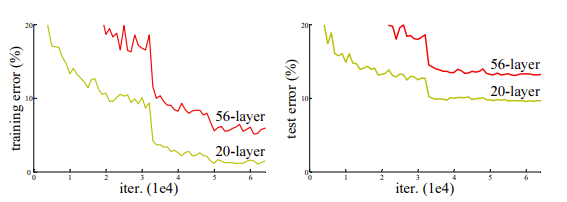
\includegraphics[width=0.45\textwidth]{figures/resnet_intro_compare.png}
        \caption{Training error (left) and test error (right) on CIFAR-10
        with 20-layer and 56-layer “plain” networks. The image was taken from the ResNet paper \cite{ResNet}.}
        \label{fig:Resnet_intro}
\end{center}
\end{figure}

\paragraph{The pitfall of vanishing gradients} The degradation phenomenon mentioned above is currently still a controversial topic, when many sources \cite{visoai, Datagen_2023,GeeksforGeeks_2023} agree that this phenomenon is rooted from the vanishing gradients problem \cite{exp_vanishing_grad_1,exp_vanishing_grad_2}. This is indeed a valid reason since the gradients would gradually decay through each individual layer in the backpropagation phase. However, the authors of ResNet argued that the vanishing gradients problem has little effect on the model causing the degradation phenomenon. “We argue that this optimization difficulty is unlikely to be caused by vanishing gradients. These plain networks are trained with BN, which ensures forward propagated signals to have non-zero variances. We also verify that the backward propagated gradients exhibit healthy norms with BN. So neither forward nor backward signals vanish.”, stated by Kaiming He et al. in their paper \cite{ResNet}. Based on this argument, they argued that the degradation phenomenon was indeed a natural dilemma arising from the action of deepening any CNN models. This argument directly opposes the effect of the vanishing gradients problem on deep models, which would require that more proof and experiments must be conducted to approve any sides. However, despite the different reasoning of the degradation phenomenon, one of the same goals of any models created till now is avoiding this problem.  

\subsubsection{Architecture}

\paragraph{Skip connections} Mathematically, defining a residual block with a skip connection as:
\[y=\uppercase{\gamma}(x) + x\]
With \(\uppercase{\gamma}(x)\) represents a generalized convolutional mapping with an activation function. The equation strictly illustrates combining input \(x\) with \(\uppercase{\gamma}(x)\) through addition expression. A skip connection is a pathway for any input feature map to flow to the output of the next layer. The intuition behind this technique resembles the process of a person reviewing a picture one more time that has not seen for a long time. Adding the input to the output feature map is believed to make the model “remember” its input, since any processing or calculation that input went through may make the output completely unrelated. Moreover, many sources of information about ResNet besides the authors agree that these skip connections will alleviate the vanishing gradients problem, hence could help the model to have a greater amount of layers.  

\begin{figure}
        \begin{center}
        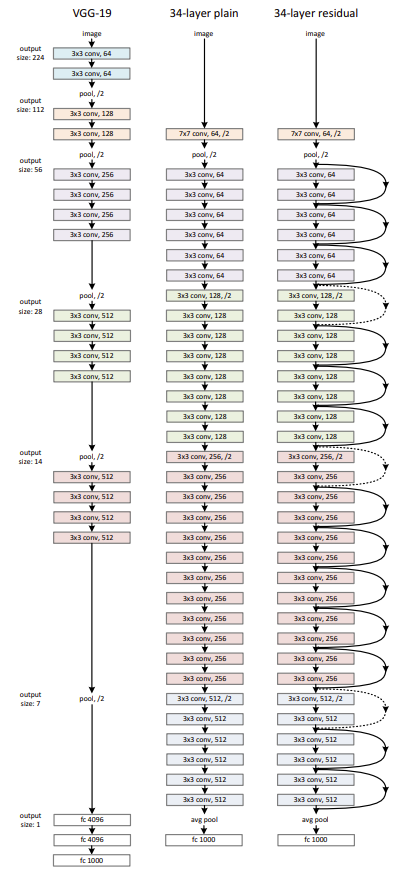
\includegraphics[width=0.4\textwidth]{figures/resnet_architecture.png}
        \caption{Architecture of ResNet compared to plain models. The image was taken from the ResNet paper \cite{ResNet}.}
        \label{fig:Resnet_architecture}
\end{center}
\end{figure}


\paragraph{The general architecture} Since skip connections can be used as an identity mapping in any CNN models, the proposed ResNet would have many layers, from 34 to 151 layers preferably. The skip connections are utilized in each layer, as shown in \ref{fig:Resnet_architecture}. The proposed ResNet model resembles the VGGNet in terms of using small kernel size for convolutional layers and stacking a sufficient amount of these layers. The skip connections can be directly used when the input and output are of the same dimensions (solid line shortcuts in \ref{fig:Resnet_architecture}). When the dimensions increase (dotted line shortcuts in \ref{fig:Resnet_architecture}), there are 2 options: (A) The shortcut still performs identity mapping, with extra zero entries padded for increasing dimensions. This option introduces no extra parameter; (B) The projection shortcut is used to match dimensions (done by 1×1 convolutions). For both options, when the shortcuts go across feature maps of two sizes, they are performed with a stride of 2.

\subsubsection{Applications}

The invention of ResNet sparks the utilization of that same structure, especially the skip connections or residual blocks, in many CNN models not only in the Computer Vision field but also a greater, older field which is Natural Language Processing. Some impactful architectures developed based on ResNet are ResNeXt \cite{ResNeXt} and DenseNet \cite{DenseNet}, where residual blocks and skip connections are implemented differently to tackle the weaknesses of ResNet. In addition, those skip connections (or preferably called identity mapping), are utilized in Transformer \cite{Transformer}, which is an evolutionary architecture that outperformed any forms of CNN in NLP. The same architecture was also widely used to create different types of Transformer models in the Computer Vision field, such as ViT \cite{ViT} or Swin \cite{Swin}. The skip connections used in Transformer sequentially made the Attention blocks in this model a new type of residual blocks.

{\small
        \bibliographystyle{ieee}
        \bibliography{bibliography.bib}
}


\end{document}